\section{Решение задачи при втором типе ограничений на управление}

В данном пункте рассмотрим задачу \eqref{eq:main_equation} с ограничением на управляющий параметр вида
$$
        v(t) \in \Omega =
        \{\,
                [v_1,\, v_2]^\T \in \R^2
                \;:\;
                v_1 \in \R,\,
                v_2 \in [m_1,\,m_2]
        \,\}.
$$
В таком случае расширенная функция Гамильтона--Понтрягина принимает вид
$$
        \hat H = \frac{1}{2}(v_1^2 + \alpha|v_1|) + \psi_1x_1 + \psi_2(v_1 - v_2x_2),
$$
максимизация которой равносильна максимизации
$$
        \frac{1}{2}(v_1^2 + \alpha|v_1|) + \psi_2(v_1 - v_2x_2) \rightarrow \max\limits_{v \in \Delta}.
$$
Тогда задача распадается на две:
$$
        \begin{aligned}
                v_1^2 + \alpha|v_1| + \psi_2v_1 & \rightarrow \max\limits_{v_1 \in \R}, \\
                -\psi_2x_2v_2 & \rightarrow \max\limits_{v_2\in[m_1,\,m_2]}.
        \end{aligned}
$$
Эти задачи имеют соответствующие решения:
$$
        v_1^* =
        \begin{cases}
                \psi_2 + \frac{\alpha}{2}, &
                \mbox{при $\psi_2<-\frac{\alpha}{2}$} \\
                0, &\mbox{при $\psi_2 \in [-\frac{\alpha}{2},\,\frac{\alpha}{2}]$} \\
                \psi_2 - \frac \alpha 2, &\mbox{при $\psi_2 > \frac \alpha 2$},
        \end{cases}
$$
$$
        v_2^* = 
        \begin{cases}
                m_2, &\mbox{при $\psi_2 x_2 < 0$}\\
                [m_1,\,m_2], &\mbox{при $\psi_2 x_2 = 0$} \\
                m_1, &\mbox{при $\psi_2 x_2 > 0$}.
        \end{cases}
$$

Полностью аналогичные рассмотренным в предыдущей параграфе рассуждения об особом режиме и первоначальном виде траектории позволяют нам записать режимы, в которых может двигаться \textit{тележка} при полученном, удовлетворяющем принципу максимума, управлении. Так как в начальный момент времени по-прежнему верна формула \eqref{eq:firstlim_psi2}, введём следующую классификацию режимов траектории:

\begin{enumerate}
        \item Пусть $A \geqslant 0$. Тогда будем говорить, что управление реализует \textit{режим акселерации}.
        \item Пусть $A < 0$.
        \begin{enumerate}
                \item Если $t_1 > T$, то будем говорить, что управление реализует \textit{режим отсутствия торможения}.
                \item Если $t_1 < T, \; t_2 > T$, то будем говорить, что управление реализует \textit{режим слабого торможения}.
                \item Если $t_2 < T, \; t_3 > T$, то будем говорить, что управление реализует \textit{режим сильного торможения}.
                \item Если $t_3 < T$, то бужем говорить, что управление реализует \textit{режим интенсивного торможения}.
        \end{enumerate}
\end{enumerate}
При такой классификации видно, что рассуждения для большинства режимов можно дословно перенести из предыдущего параграфа (или, как в случае режима сильного торможения, добавить дополнительную проверку). В связи с этим проведём рассуждения только для режимов, отличающихся от рассмотренных ранее.

%%%%%%%%%%%%%%%%%%%%%%%%%%%%%%%%%%%
%                                 %
%  Режим интенсивного торможения  %
%                                 %
%%%%%%%%%%%%%%%%%%%%%%%%%%%%%%%%%%%
\subsection{Режим интенсивного торможения}

\begin{figure}[h]
        \hfill
        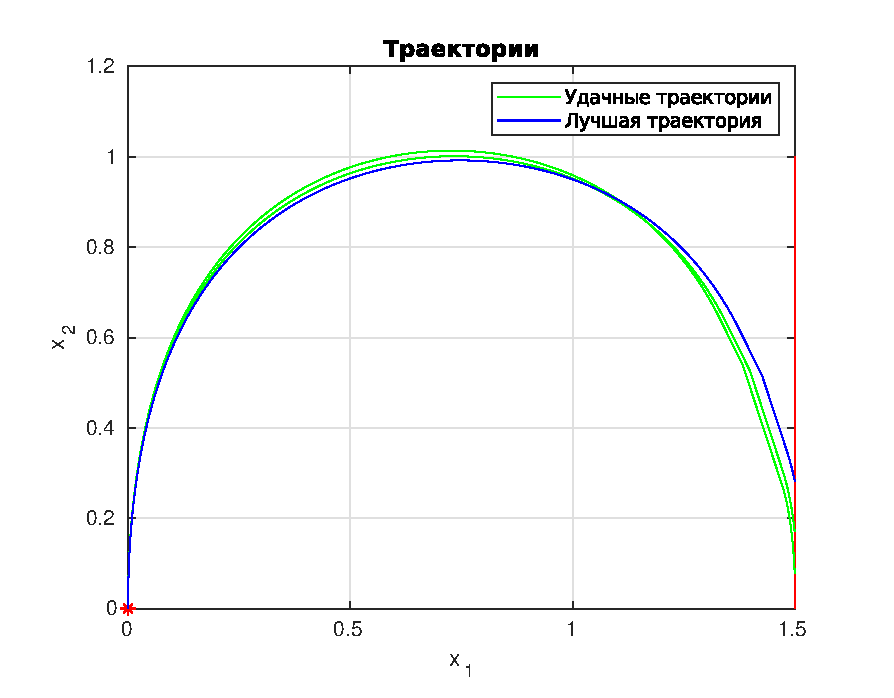
\includegraphics[width=70mm]{second/int2.eps}
        \hfill
        \hfill
        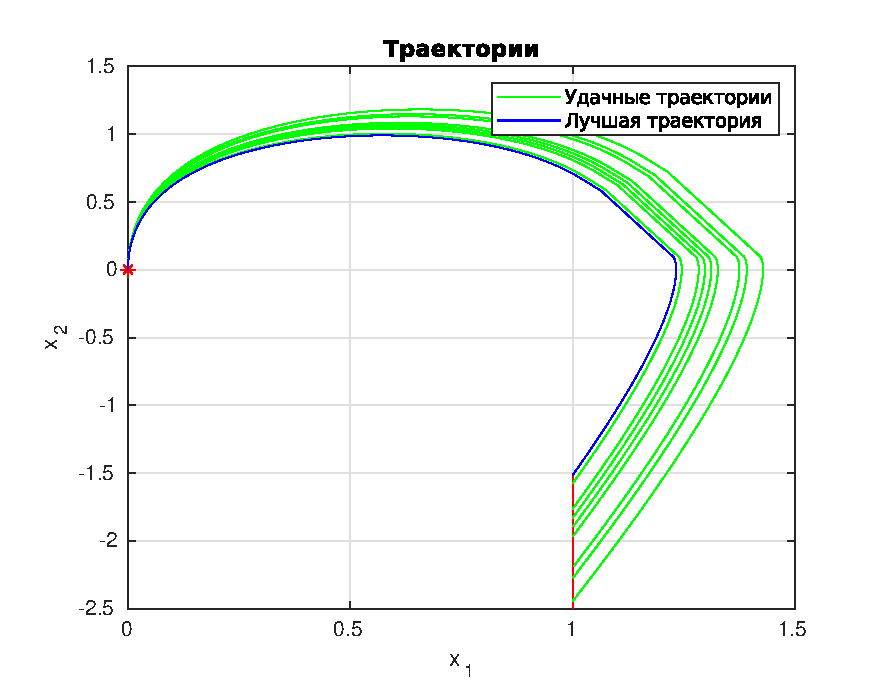
\includegraphics[width=70mm]{second/int1.eps}
        \hfill
        \caption{Перебираемые траектории в режиме интенсивного торможения для двух разных постановок задач. Слева целевое множество находистя выше оси абсцисс, справа --- ниже.}
\end{figure}

На промежутке времени $t_2 \leqslant t \leqslant T$ вторая компонента сопряжённой системы имеет вид:
$$
        \psi_2(t)
        =
        -\psi_1^0 \int\limits_{t_2}^{t} e^{m_2(t - \tau)}\,d\tau
        =
        \frac{m_1}{m_2}B\left( 1 - e^{m_2(t - t_2)} \right).
$$
Откуда получаем, что
$$
        t_3 = t_2 + \frac 1 {m_2} \ln \left(
                \frac{\alpha m_2}{2m_1B} + 1
        \right).
$$

Теперь можем получить уравнения, описывающие поведение \textit{тележки} на отрезке времени $t_3 \leqslant t \leqslant T$:
\begin{multline}
        x_2(t) = x_2^3 e^{m_2(t_3 - t)} + \int \limits_{t_3}^t e^{m_2(\tau - t)} \left(\frac{m_1}{m_2}B + \frac{\alpha}{2} + \frac{m_1}{m_2}Be^{m_2(\tau - t_2)}\right)\,d\tau = 
        \\
        =  x_2^3 e^{m_2(t_3 - t)} + \frac 1 {m_2} \left[
        \left( \frac{m_1}{m_2}B + \frac\alpha 2\right) \left( 1 - e^{m_2(t_3 - t)} \right) - \right.
        \\
        \left.
        - \frac{\alpha m_1}{2m_2}B\left( e^{m_2(t-t_2)} - e^{m_2(2t_3-t-t_2)}\right)\right],
\end{multline}
\begin{multline}
        x_1(t) = x_1^3 + \int\limits_{t_3}^t x_2(\tau)\,d\tau = x_1^3 + \frac{x_2^3}{m_2} \left(1 - e^{m_2(t_3 - t)}\right) +
        \\
        + \frac{1}{m_2} \left[ \left( \frac{m_1}{m_2}B + \frac \alpha 2 \right)\left( t - t_3 - \frac{1}{m_2} \left( 1 - e^{m_2(t_3 - t)}\right)\right) - \right.
        \\ 
        \left.
        - \frac{\alpha m_1}{2m_2^2}B\left( e^{m_2(t-t_2)} - 2e^{m_2(t_3-t_2)} + e^{m_2(2t_3-t-t_2)}\right)\right].
\end{multline}

Таким образом, мы можем устроить перебор по времени первого и втрого переключений $0 < t_1 < T$, $t_1 < t_2 < T$ и решать задачу так же, как мы делали это в режиме сильного торможения. В случае если найденное по формуле время третьего переключения оказалось меньше заданного конечного времени $T$, мы можем построить конечную часть траектории по вышеприведённым формулам.





